\section{Comparison with a boundary element code}
\label{sec:cost}

In this section we compare accuracy against wall time for the MFS and the boundary element library Bempp \cite{betcke2021} (\autoref{fig:costall}, \autoref{tab:summary} and \autoref{tab:cubeends}). For exterior scattering in a homogeneous medium by bodies with sharp edges and tips, the weakly singular Galerkin electric-field integral equation (EFIE) is the most direct benchmark: unlike volumetric finite-element or finite-difference schemes, which mesh an artificial exterior box with perfectly matched layers and incur numerical dispersion and truncation reflections, it discretises $\Gamma$ alone and satisfies the radiation condition analytically; and unlike magnetic-field or smooth-surface Nystr\"om integral equations \cite{burbano2026}, it applies directly at sharp wedges and conical vertices \cite{rao1982,bespalov2010}. At these electrical sizes, dense direct factorisation also outperforms unpreconditioned GMRES (which stagnates on edge-graded EFIE matrices) and avoids the sixfold barycentric dual-mesh overhead of Calder\'on preconditioning. To run lowest-order Bempp at its best, we used its OpenCL dense backend, graded the polyhedral meshes towards the edges, scanned gradings, quadrature orders and mesh sizes to form its \emph{lower envelope} (retaining runs at least $3\%$ more accurate than every faster run), and equipped it with the exact mirror, half-turn and rotational symmetries of the MFS (\ref{app:bempp}), speeding Bempp up by three to twenty times without loss of accuracy. Direct comparisons were timed alternately on an idle machine, keeping the minimum time of repeated runs.

\begin{figure}[htbp]
  \centering
  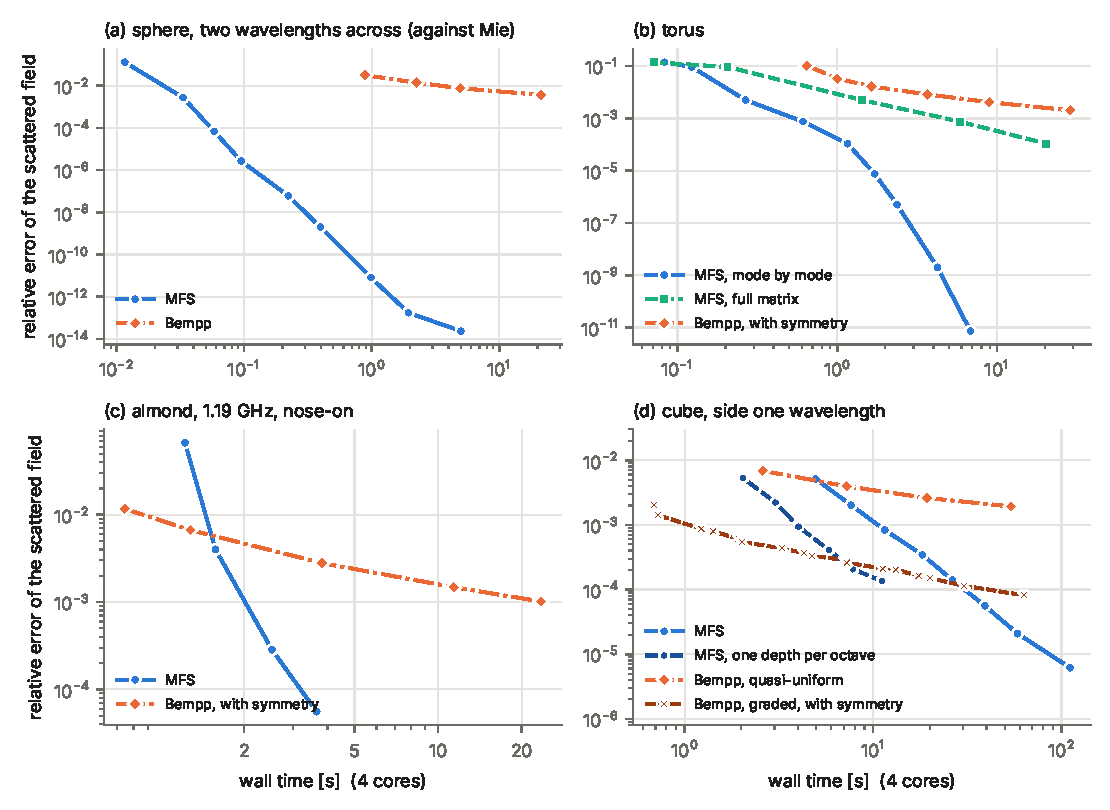
\includegraphics[width=\textwidth]{fig_cost_all.pdf}
  \caption{Error of the scattered field against wall time on two cores for the MFS and for Bempp. (a) Unit sphere at $k = 2\pi$, error against the Mie series. (b) Torus ($R = 1$, $a = 0.5$) at $k = 2\pi$, difference from the finest MFS run; both codes use the rotational symmetry. (c) NASA almond at $1.19$\,GHz, nose-on, difference from the finest MFS layout; both codes use the two mirror planes. (d) Unit cube at $k = 2\pi$, difference from the finest MFS layout (\autoref{sec:cuberesults}): the MFS from $J = 3$ with two depths and one depth per octave (combined lower envelope shaded), Bempp on quasi-uniform meshes, and the lower envelope of symmetric graded Bempp up to its $8$\,GB memory limit.}
  \label{fig:costall}
\end{figure}

\subsection{Smooth bodies and the almond}

On the sphere, the torus and the nose-on almond at $1.19$\,GHz, the MFS reaches errors between $5.6\times10^{-5}$ and $3.5\times10^{-14}$ in ten seconds or less, whereas Bempp's largest meshes reach $2.6\times10^{-4}$ to $2.3\times10^{-3}$ in $130$ to $329$ seconds (for the torus and almond the reference is the finest MFS layout, independently verified in Sections~\ref{sec:torus} and~\ref{sec:almond}). Because lowest-order RWG elements on flat triangles of size $h$ converge like $O(h^2)\propto N_u^{-1}$, this gap at high accuracy against a spectral or root-exponential method is expected, and curved, higher-order boundary elements \cite{bespalov2010} would narrow it. The same contrast appears at $3.5$\,GHz (three wavelengths long), where layouts $5{:}2$ and $6{:}3$ on the almond reach $2.8\times10^{-4}$ in $4.3$\,s and $4.6\times10^{-5}$ in $8.4$\,s, against $3.1\times10^{-3}$ in $17$\,s and $1.1\times10^{-3}$ in $133$\,s for Bempp.

Closer to the surface $\Gamma$, the difference between the two methods grows sharply (\autoref{fig:nearfield}). Because the MFS field is a finite sum of smooth interior dipole fields, it is evaluated identically everywhere outside $\Omega$: on the sphere it stays below $3\times10^{-7}$ ($N = 400$) and $10^{-13}$ ($N = 1200$) right up to $\Gamma$ (and up to $\Gamma$ away from polyhedral edges, \autoref{fig:edgeresidual}). Evaluating a boundary element field within one triangle width of $\Gamma$, in contrast, makes the surface integral nearly singular. Without specialised near-singular quadrature, Bempp's error on the $h = 0.07$ sphere mesh stays at $4\times10^{-3}$ down to distance $0.03$, but rises to $8\%$ at $0.01$ and exceeds $100\%$ at $10^{-3}$.

\begin{table}[tbp]
  \centering
  \caption{Selected runs of \autoref{fig:costall}(a)--(c): whole-body unknowns (Total), unknowns solved for the incident wave after symmetry reduction (Solved), wall time and error, measured as in the figure. On the torus, the axial wave excites two azimuthal Fourier modes ($m = \pm1$); on the almond, the nose-on wave excites one of the four mirror-symmetry classes (\ref{app:bempp}). The cube is summarised in \autoref{tab:cubeends}, and the regular tetrahedron in \autoref{sec:tetrahedron}.}
  \label{tab:summary}
  \small
  \begin{tabular}{llrrrl}
    \toprule
     &  & \multicolumn{2}{c}{Unknowns} &  &  \\
    \cmidrule(lr){3-4}
    Shape & Method & Total & Solved & Time [s] & Error \\
    \midrule
\tablebody{summary}
    \bottomrule
  \end{tabular}
\end{table}

\begin{figure}[htbp]
  \centering
  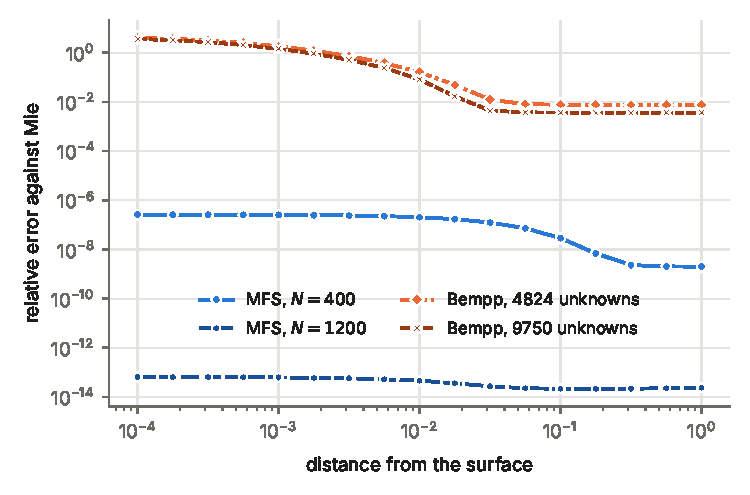
\includegraphics[width=0.68\textwidth]{fig_sphere_nearfield.pdf}
  \caption{Unit sphere, $k = 2\pi$: error of the scattered field against the Mie series as a function of the distance from the surface, for the MFS ($R_s = 0.5$) with $1200$ and $3600$ unknowns ($N = 400$ and $1200$ sources) and for Bempp with $4824$ and $9750$ unknowns (triangles of size $0.1$ and $0.07$, below which fixed-order quadrature loses accuracy).}
  \label{fig:nearfield}
\end{figure}

\subsection{The polyhedra and what the comparison shows}

On the cube, default quasi-uniform Bempp meshes still leave $2\times10^{-3}$ error after four minutes ($262$\,s), whereas edge-graded meshes are close at low accuracy (\autoref{tab:cubeends}, Figures~\ref{fig:cubecases} and~\ref{fig:costall}(d)). At the high-accuracy end, Bempp's largest mesh fitting in memory ($41472$ unknowns, $636\text{--}665$\,s) is overtaken by the MFS in $35\text{--}98$\,s ($14$\,s to $7.1\times10^{-5}$ at $k = 2\pi$ with one depth per octave), and the MFS continues past that $8$\,GB ceiling to $2.1\times10^{-5}$ in $83$\,s and $6.8\times10^{-6}$ in $123$\,s ($k = 2\pi$, standard wave). On the regular tetrahedron (\autoref{sec:tetrahedron}), the MFS envelope lies below symmetric graded Bempp at every accuracy, reaching $1.5\times10^{-3}$ in $4.4$\,s (versus $1.8\times10^{-3}$ in $6.8$\,s) and $1.0\times10^{-4}$ in $36$\,s (versus $2.2\times10^{-4}$ in $267$\,s). Near $10^{-3}$ on the cube, the MFS is faster for the standard wave at $k = 2\pi$ ($3.1$\,s versus $3.8$\,s), about $1.3\times$ for the general wave ($6.0$\,s versus $4.5$\,s), and twice as fast at $k = 4\pi$ and $6\pi$ ($6.3$\,s versus $12$\,s, and $15$\,s versus $34$\,s).

Between these two ends, the crossover moves towards coarser tolerances as frequency grows: from $4.0\times10^{-4}$ and $3.5\times10^{-4}$ (standard and general waves) at one wavelength to $8.0\times10^{-4}$ and $1.1\times10^{-3}$ at two and three wavelengths for two depths per octave alone, and to $9.8\times10^{-4}$, $7.7\times10^{-4}$, $3.7\times10^{-3}$ and $3.2\times10^{-3}$ once the fast one-depth variant is included ($1.3\times10^{-4}$ in $10.3$\,s against $86\text{--}149$\,s for Bempp at $k = 2\pi$).

\begin{table}[htbp]
  \centering
  \caption{Unit cube, both ends of the comparison. Left: the most accurate run of Bempp (on the $41472$-unknown mesh) and the first MFS run with a smaller error, each with its wall time. Right: wall time of the fastest run of each code with an error of about $10^{-3}$ (at most $1.2\times10^{-3}$; for the MFS, the faster of one and two depths per octave is taken).}
  \label{tab:cubeends}
  \small
  \setlength{\tabcolsep}{4pt}
  \begin{tabular}{llrlrrr}
    \toprule
     & \multicolumn{2}{c}{Bempp, most accurate} & \multicolumn{2}{c}{MFS, first better} & \multicolumn{2}{c}{Time [s] for $10^{-3}$} \\
    \cmidrule(lr){2-3}\cmidrule(lr){4-5}\cmidrule(lr){6-7}
    Case & Error & [s] & Error & [s] & Bempp & MFS \\
    \midrule
\tablebody{cube_ends}
    \bottomrule
  \end{tabular}
\end{table}

Overall, the MFS is faster across the tested range on smooth bodies and the regular tetrahedron, below $10^{-2}$ on the almond ($1.19$ and $3.5$\,GHz), and below $8\times10^{-4}\text{--}4\times10^{-3}$ across all four cube cases. Above those coarse cube tolerances, graded Bempp is competitive or $1.3\text{--}2$ times faster (oblique wave), whereas below them the gap opens rapidly: Bempp's effective algebraic order $p$ in $\varepsilon\propto N_u^{-p}$ drops from $1.4$ on coarse meshes to $0.8\text{--}1$ on fine ones, while that of the MFS rises from $2.7$ to $4.8$ (\autoref{fig:cubeconv}).
